\documentclass{beamer} %

 

%%%BASICS

\usepackage[utf8]{inputenc}

\usepackage{csquotes}

 

%%%START THEME SETTINGS

\usetheme{Dresden}

\usecolortheme{beaver}

\usefonttheme{professionalfonts}

\setbeamertemplate{itemize item}{\color{red}$\blacksquare$}

%%%END THEME SETTINGS

 

%%%START APA

\usepackage[british]{babel}

\usepackage[backend=biber,style=apa]{biblatex}

\usepackage{graphicx}

\graphicspath{ {./Images/} }

\DeclareLanguageMapping{british}{british-apa}

\addbibresource{references.bib}

%% APA citing

%% \cite{t} - Uthor und Richter, 2010

%% \textcite{t} - Uthor und Riter (2010)

%% \parencite{t} - (Uthor & Riter, 2010)

%% \parencite[Chapt.~4]{t} - (Uthor & Riter, 2010, S. 15)

%%%END APA

 

 

\title[Comparisons of Health, Wellness and Food Accessibility in the United States]{Comparisons of Health, Wellness and Food Accessibility in the United States}

\institute[UNL]{University of Nebraska-Lincoln}

\author{Rene Ingersoll, Kuljit Bhatti, Alyssa Grube}

 

\date{\today}

 

\usepackage{Sweave}
\begin{document}
\input{Slides-concordance}

 

\begin{frame}

                \titlepage

\end{frame}

 

%------------------------------------------------------

 

 

\begin{frame}

 

\end{frame}

 

\begin{frame}{Spatial Analysis: Introduction}
\setbeamertemplate{itemize items}[triangle]
  \begin{itemize}
  \item Question 1: Does obesity correlate to areas with easy access to food?
  \item Question 2: Is access to food effected by if the region is urban or rural?
  \end{itemize}
\end{frame}

\begin{frame}{Data}
\setbeamertemplate{itemize items}[triangle]
\begin{itemize}
  \item Food Access Data
    \begin{itemize}
        \item Percent of population that is obese (2017)
        \item Percent of population with low access to food (2015)
    \end{itemize}
    \item Census Data
        \begin{itemize}
            \item Shape-files: State, County, Urban Clusters
        \end{itemize}
\end{itemize}
\end{frame}

%------------------------------------------------------

\begin{frame}{Looking at data Spatially}
\begin{itemize}
    \item Constructing Maps
        \begin{itemize}
            \item Packages: ggplot2, sf
            \item Overlaid geometry of the 2-3 spatial scales
            \item centered the map on the US or state by adjusting coordinates
        \end{itemize}
    \item Urban vs. Rural
        \begin{itemize}
            \item According to the US Census Bureau: "There are two types of urban areas: urbanized areas (UAs) that contain 50,000 or more people and urban clusters (UCs) that contain at least 2,500 people, but fewer than 50,000 people"
        \end{itemize}
\end{itemize}
\end{frame}

%------------------------------------------------------

\begin{frame}{Obesity and Food Access Maps}
\begin{figure}
   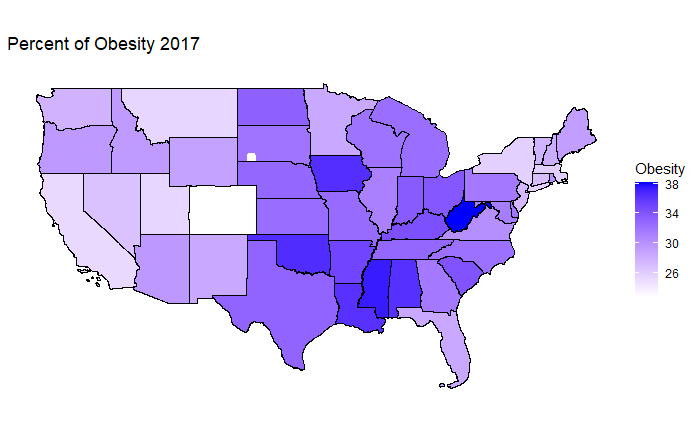
\includegraphics[width=0.5\textwidth]{Obesity_Map.jpg}
   \hfill
   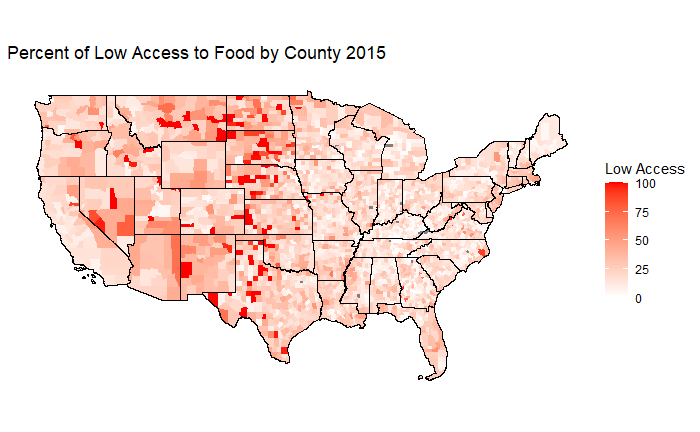
\includegraphics[width=0.5\textwidth]{Food_Access.jpg}
\end{figure}
\end{frame}


%------------------------------------------------------ 
 
\begin{frame}{Comparing Urban and Rural}
\begin{figure}
   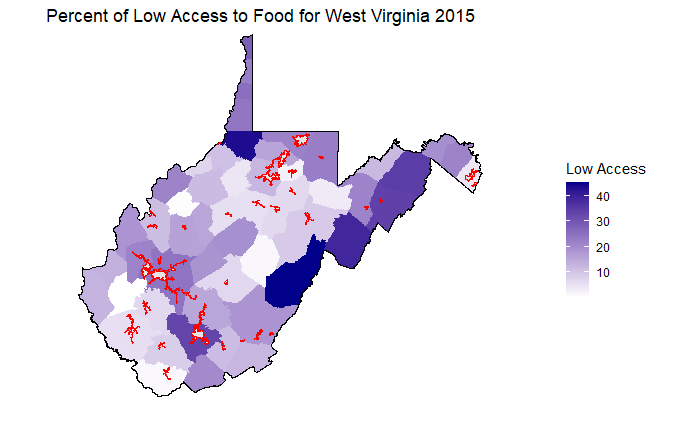
\includegraphics[width=0.475\textwidth]{WV_Map.jpg}
   \hfill
   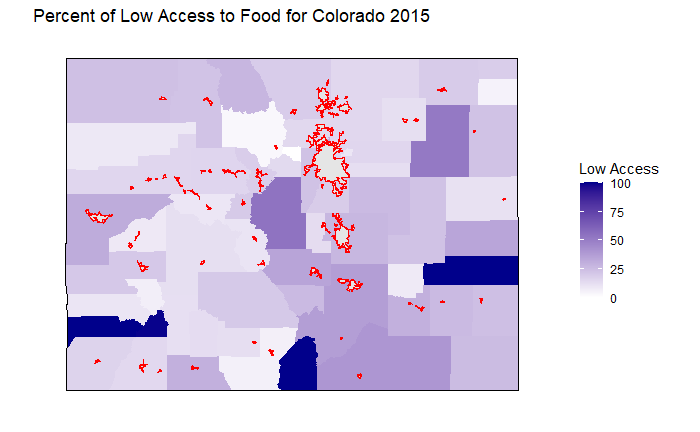
\includegraphics[width=0.475\textwidth]{CO_Map.jpg}
\end{figure}
\end{frame}


%------------------------------------------------------ 
 
 
\begin{frame}{Continuation}
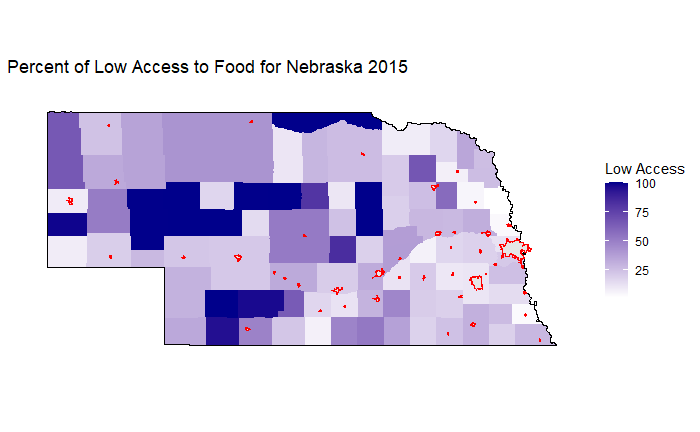
\includegraphics{NE_Map.jpg}
\end{frame}
 

\printbibliography

 

\end{document}
